\chapter{Dostupné platformy}

Pro \legoEV{} existuje mnoho vývojových platforem. 
Většinou se jedná o~specificky navržené programovací API ve~spojení s~vývojovým prostředím. 
Tyto platformy většinou využívají oficiální systém v~\EVthree{}, ale jsou i~platformy s~vlastním operačním systémem. 
V~tomto textu bude popsán jen výběr těch nejzajímavějších. % platforem. 

\section{Originální prostředí od \lego}

V rámci této podkapitoly bude rozebrán samotný operační systém na \EVthree{} a také vývojové prostředí určené pro tvorbu a ladění programů. 
\lego{} si pro \EVthree{} vytvořilo vlastní operační systém postavený na linuxovém jádru \cite{legoMindstormsEV3_fw-dev-kit}. 
Uvnitř systému běží virtuální stroj, který zpracovává byte-code uživatelské aplikace. 
Byte-code je vytvořen ve~vývojovém prostředí na PC a~odeslán do \brick{\it u}. 

Celý systém s~vývojářskými nástroji a~dokumentací je volně k~dispozici na~webu \lego{}~\cite{legoMindstorms_download}. Díky tomu, že~\lego{} uvolnilo zdrojové kódy mohli vzniknout alternativní systémy pro~\EVthree{} jako~\evThreeDev{} nebo \evRT. 

\subsection{\legoSW{}}

\begin{figure}[h]
	\centering
	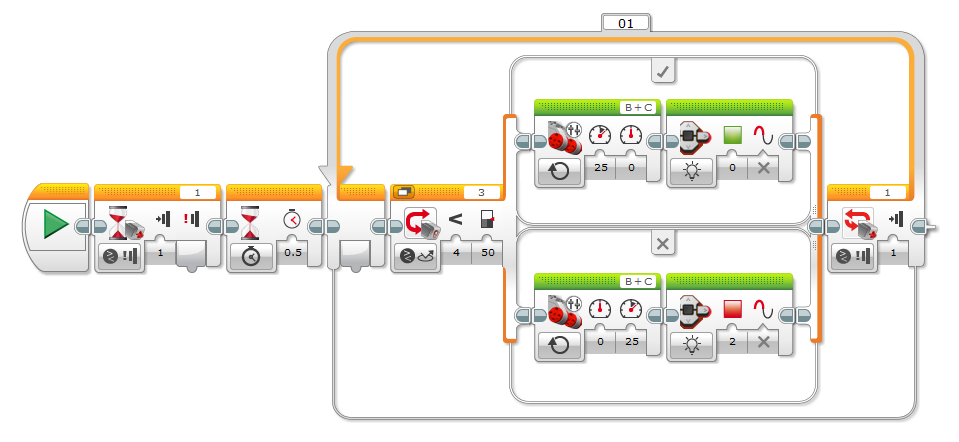
\includegraphics[width=0.99\textwidth]{images/lego-soft/lego-soft_robotut_switch-touch+motors+leds.png}
	\caption{Ukázka programovacích bloků v \legoSW}
	\label{fig:lego-soft_example-blocks}
\end{figure}

\legoSW{} je~vývojářský program, který \lego{} k~\EVthree{} zdarma poskytuje. 
Jedná se o~software, který \lego{} vytvořilo ve~spolupráci s~firmou \NI{} a~je postavený na~základen programu \labview{}. 
\lego{} s~\NI{} již~spolupracovalo na předešlých vývojářský programech. % pro~\legoM{}. %  a~proto ani tentokrát neudělalo výjimku.  
Program se~snaží působit jako profesionální vývojové a~laboratorní studio, což se~mu celkem daří.
Nabízí celou řadu funkcí od modulu pro programování, přes tvorbu různých experimentů až~po přípravy interaktivních návodů a~průvodců programováním v~tomto prostředí.



V~režimu tvorby programu jsou hlavním stavebník kameny \EVblocks, které se ve~formě diagramů skládají do podoby výsledného programu (obrázek \ref{fig:lego-soft_example-blocks}).
Bloky jsou rozděleny do~několika skupin (akční, tok programu, senzory, datové operace, pokročilé a~vlastní), které se liší i~svoji barvou. 
Pomocí těchto bloků lze řídit tok programu (podmínky, cykly, čekání a vlákna), pracovat s~proměnnými, obsluhovat senzory, provádět matematické operace a~nebo i~využívat vlastní bloky.

\begin{figure}[h]
	\centering
	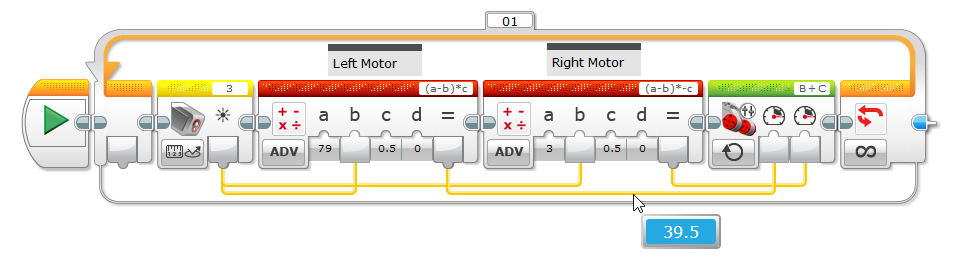
\includegraphics[width=\textwidth]{images/lego-soft/lego-soft_live-debuging_line-advance.png}
	\caption{Ukázka debugování za běhu programu}
	\label{fig:lego-soft_live-debuging_line-advance}
\end{figure}

Vše je pěkně graficky zpracováno a~působí to~jako jednotný celek. 
Při běhu programu lze~sledovat jeho tok (kde v diagramu se program nachází) a~nebo si i~zobrazit aktuální stav (hodnotu proměnné, výsledek matematické operace, výstupní data ze~senzoru, \dots). 
Ukázku si~lze prohlédnout na obrázku \ref{fig:lego-soft_live-debuging_line-advance}, kde je vidět hodnota 39.5 odpovídající výsledku výpočtu výkonu pro levý motor v~závislosti na~naměřené hodnotě od barevného senzoru.
Zároveň je podle šrafování vrchní lišty bloků vidět, že~program aktuálně probíhá v~daném cyklu.

Pro práci s~\brick{\it em} je k~dispozici modul {\it Správa hardwaru}, kde lze zjisti například informace o \brick{\it u} (jméno, stav baterie, verze firmwaru, obsazenost paměti)

\begin{figure}[h]
	\begin{minipage}[b]{.45\textwidth}
		\centering
		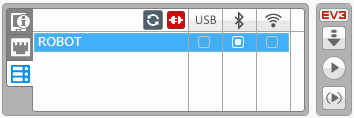
\includegraphics[width=\textwidth]{images/lego-soft/lego-soft_brick-manager_connected.png}
		\caption{Správa připojení k \brick{\it u}}
		\label{fig:lego-soft_brick-manager-connected}
	\end{minipage}
	\hfill
	\begin{minipage}[b]{.45\textwidth}
		\centering
		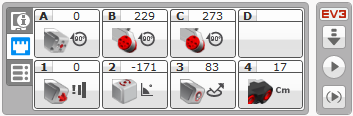
\includegraphics[width=\textwidth]{images/lego-soft/lego-soft_brick_port-view.png}
		\caption{Informační panel s porty}
		\label{fig:lego-soft_brick_port-view}
	\end{minipage}
\end{figure}

Nevýhody \legoSW:
\renewcommand{\labelitemi}{$-$}
\begin{itemize}[noitemsep]\itemsep2pt
	\item náročný na hardware počítače
	\item větší programy se stávají nepřehledné a špatně se v nich orientuje a hledají chyby
	\item nelze editovat proměnné ani uživatelské bloky
	\item debugovací režim nefunguje uvnitř uživatelských bloků
	\item při rozsáhlejších programech přestává prostředí fungovat (zamrzává a padá)
	\item není dostupný na Linuxu a není open-source
\end{itemize}

Nevýhody operačního systému v \brick{\it u}:  %na \lego:
\begin{itemize}[noitemsep]\itemsep2pt
	\item dlouhé zapínání a vypínání \brick{\it u}
	\item nekonzistentní chování programů v režimu, kdy je \brick{} připojen k PC a kdy ne
	\item značně pomalé zpracovávání některých operací (\dots)
	\item není real-timový a časování jednotlivých operací tedy není garantováno
\end{itemize}

\begin{figure}[h]
	\centering
	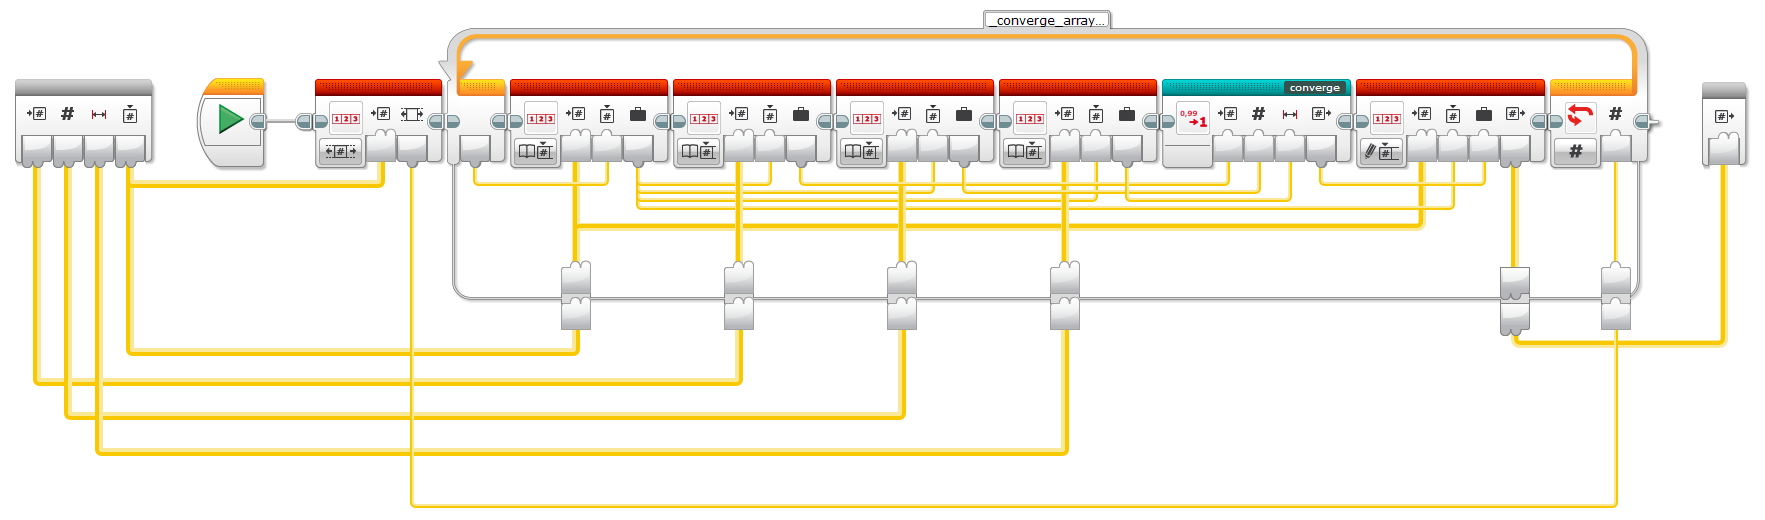
\includegraphics[width=\textwidth]{images/lego-soft/lego-soft_legolib_converge_array.png}
	\caption{Ukázka debugování za běhu programu}
	\label{fig:lego-soft_live-debuging_line-advance}
\end{figure}


\begin{figure}[h]
	\centering
	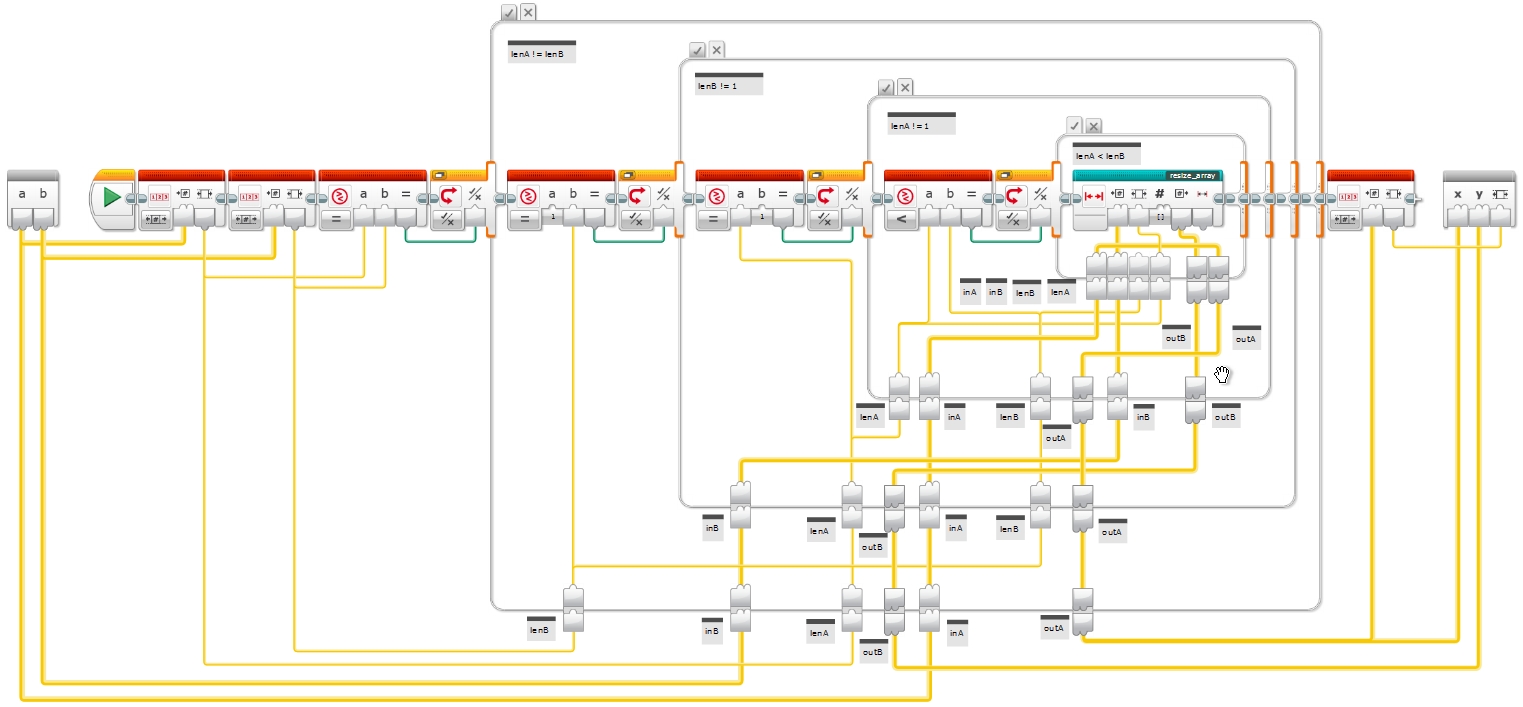
\includegraphics[width=\textwidth]{images/lego-soft/lego-soft_legolib_match_array_length.png}
	\caption{Ukázka debugování za běhu programu}
	\label{fig:lego-soft_live-debuging_line-advance}
\end{figure}



 